%! Author: Facundo Bautista Barbera
%! Date: 2025-09-22
%! TEX root = main.tex

\documentclass{article}

\usepackage{amsmath}
\usepackage[utf8]{inputenc}
\usepackage{listings}
\usepackage{xcolor}
\usepackage{graphicx}
\usepackage{selnolig}

\definecolor{codegreen}{rgb}{0,0.6,0}
\definecolor{codegray}{rgb}{0.5,0.5,0.5}
\definecolor{codepurple}{rgb}{0.58,0,0.82}
\definecolor{backcolour}{rgb}{0.95,0.95,0.92}

\lstdefinestyle{mystyle}{
    backgroundcolor=\color{backcolour},
    commentstyle=\color{codegreen},
    keywordstyle=\color{magenta},
    numberstyle=\tiny\color{codegray},
    stringstyle=\color{codepurple},
    basicstyle=\ttfamily\footnotesize,
    breakatwhitespace=false,
    breaklines=true,
    captionpos=b,
    keepspaces=true,
    numbers=left,
    numbersep=5pt,
    showspaces=false,
    showstringspaces=false,
    showtabs=false,
    tabsize=2
}

\lstset{style=mystyle, inputencoding=utf8}

\title{main}
\author{Facundo Bautista Barbera}
\date{\today}

\begin{document}
\maketitle

\section*{Actividad}

Para esta actividad creamos una simulación para una cadena de Markov.
Las probabilidades del clima de una situación hipotetica se muestran en la siguiente matriz:

$
	p =
	\begin{bmatrix}
		0.8 & 0.2 \\
		0.6 & 0.4
	\end{bmatrix}
$

\section*{Código de la simulación}

A continuación se muestra el código en Python utilizado para la simulación de Monte Carlo.

\begin{lstlisting}[language=Python]
from random import random
import matplotlib.pyplot as plt

iterations = 70000
current_state = "dry"

states = [current_state]

for _ in range(1, iterations):
    random_num = random()

    if current_state == "dry":
        if random_num <= 0.8:
            current_state = "dry"
        else:
            current_state = "rain"
    else:  # current_state == "rain"
        if random_num <= 0.6:
            current_state = "dry"
        else:
            current_state = "rain"

    states.append(current_state)


dry_counts = []
count_dry = 0

for i, state in enumerate(states, start=1):
    if state == "dry":
        count_dry += 1
    dry_counts.append(count_dry / i)


# Plot
plt.figure(figsize=(10, 5))
plt.plot(
    range(1, iterations + 1),
    dry_counts,
    label="Relative frequency of Dry",
)
plt.xlabel("iterations")
plt.ylabel("relative frequency")
plt.legend()
plt.grid(True)
plt.savefig("mc_simulation.png")

absolute_frequency = count_dry
relative_frequency = dry_counts[-1]

print(f"Frecuencia absoluta en la \'ultima iteraci\'on: {absolute_frequency}")
print(f"Frecuencia relativa en la \'ultima iteraci\'on: {relative_frequency}")
\end{lstlisting}

\section*{Resultados}

Frecuencia absoluta en la \'ultima iteraci\'on: 52493

Frecuencia relativa en la \'ultima iteraci\'on: 0.7499

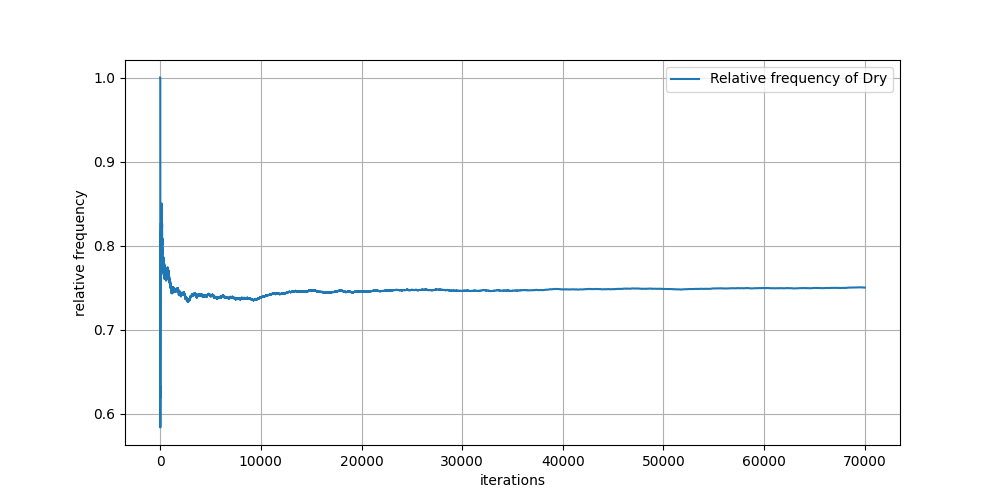
\includegraphics[width=\linewidth]{mc_simulation.png}

\end{document}
